\documentclass[11pt,a4paper]{article}

%\input{config}
\usepackage[czech]{babel}
\usepackage[utf8]{inputenc}
\usepackage{times}
\usepackage{url}
\usepackage[textwidth=15.2cm,textheight=23cm]{geometry}
\usepackage{xcolor}
\usepackage{color}
\usepackage[unicode, colorlinks,hyperindex,plainpages=false,pdftex]{hyperref}
\usepackage{graphicx}
\usepackage{float}
\usepackage{multirow}
\usepackage{amssymb}

\usepackage[bf]{caption}

\pdfcompresslevel=9

\newcommand{\myincludegraphics}[4]{
  \begin{figure}[!h]
  \centering
  \includegraphics[#1]{#2}
  \caption{#3.} \label{#4}
  \end{figure}
}

% titulní stránka a obsah
\newcommand{\titlepageandcontents}{
  % credits for template go to: Martin Striz
\begin{titlepage}

\vspace*{1cm}

\begin{figure}
  \centering
  
\includegraphics[height=6cm]{images/fit.pdf}
\end{figure}

\vspace*{5mm}

\begin{center}
\begin{Large}
Projekt do předmětu FYO -- Fyzikální optika
\end{Large}
\end{center}

\vspace*{5mm}

\begin{center}
\begin{Huge}
Fourierovská optika. Úprava obrazu.\\
\end{Huge}
\end{center}

\vspace*{1cm}

\begin{center}
\begin{Large}
\today
\end{Large}
\end{center}

\vfill

\begin{flushleft}
\begin{large}
\begin{tabular}{ll}

\bf Řešitel:\hspace{3mm} 
& Jan Wozniak (\verb_xwozni00@stud.fit.vutbr.cz_) \\
& Fakulta Informačních Technologií \\
& Vysoké Učení Technické v~Brně

\end{tabular}
\end{large}
\end{flushleft}

\end{titlepage}

% vim:set ft=tex expandtab enc=utf8:


  \pagestyle{plain}
  \pagenumbering{roman}
  \setcounter{page}{1}
  %\tableofcontents

  \newpage
  \pagestyle{plain}
  \pagenumbering{arabic}
  \setcounter{page}{1}
}









\begin{document}
\titlepageandcontents
\section{Úvod}
Obraz, jak jej vnímáme, může být reprezentován jako diskrétní dvourozměrná funkce $f[i,j]$.
Pro zobrazení v počítači lze rovněž pochopit tuto funkci jako matici, kde hodnoty $i$ a $j$ 
označují index řádku, resp. sloupce, této matice a hodnota prvku matice charakterizuje míru jasu pro daný
prvek matice -- pixel. V připadě, že se jedná o černobílý obrázek, jas je tvořen skalární hodnotou, 
velmi často 8 bitové hloubky, barevné hodnoty jsou reprezentovány pomocí složených datových typů
v konkrétním barevném modelu, tuto strukturu lze chápat jako vektorovou hodnotu. 

Existuje mnoho způsobů jak se zabývat optikou, optickým zobrazováním a úpravami obrazu.
Jeden z moderních pohledů spočívá ve využití Fourierovy transformace, která slouží k převodu
obrazu z prostorové domény do domény frekvenční. Této konverze lze docílit jak digitálně
díky matematickým vztahům ale analogickými postupy i s využitím fyzikálních zákonů a čočky.

\subsection{Historie}



\section{Fyzikální principy}
\begin{figure}[h!]
\centering
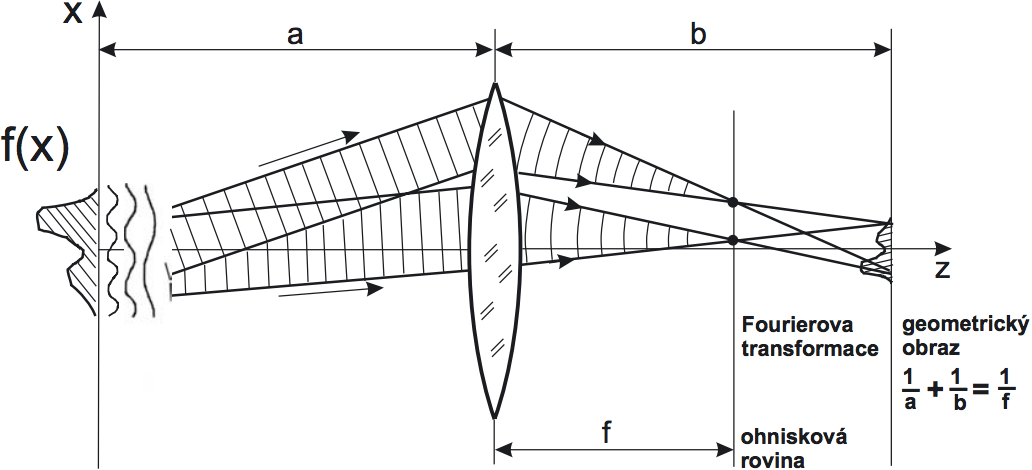
\includegraphics[width=11cm]{images/ft-cocka.png}
\caption{Optické zobrazování z hlediska Fourierovy transformace.}
\label{lcpstack}
\end{figure}




\section{Matematické principy}
Tento projekt se zabývá úpravami obrazu, a jak bylo řečeno v úvodu, obraz lze pochopit jako 2D diskrétní 
signál, proto vztahy pro Fourierovu transformaci budou popsány rovněž z pohledu dvourozměrného signálu.

\begin{equation}
F[k,l] = \sum_{m=0}^{N}{\sum_{n=0}^{N}{f[m,n]e^{(-i)\frac{2\pi km}{N}}\cdot e^{(-i)\frac{2\pi ln}{N}}}}
\label{dft}
\end{equation}

Kde $N$ jsou rozměry obrazu v pixelech, tedy $N^2$ dává celkový počet pixelů, a hodnoty $k$ a $l$ 
jsou diskrétní pozice v obrazu. 

Neboť velmi častou aplikací pro Fourierovu transformaci je frekvenční filtrace, je vhodné uvést vztah 
pro konvoluci.
\begin{equation}
g[m,n] = \sum_{k=0}^{N}{\sum_{l=0}^{N}{f[k,l]\cdot h[m-k, n-l]}}
\label{konvoluce}
\end{equation}


\section{Aplikace}
Mimo zpracování obrazu je Fourierova transformace používaná v mnoha dalších oblastech jako například
řešení parciálních diferenciálních rovnic, rychlé násobení dvou velkých čísel. Nejlépe lze pozorovat
důležitost Fourierovy transformace na faktu, že v dnešní době velká řada moderních DSP procesorů obsahuje
instrukce pro optimalizaci výpočtů rychlé Fourierovy transformace a zároveň existuje široké spektrum
paralelních implementací urychlujících tento výpočet pomocí SIMD instrukční sady na běžných CPU.

\subsection{Analýza složitosti}
Pro ideální využití Fourierovy transformace je vhodné znát i složitost výpočtu. Aby bylo  možné se
abstrahovat od konkrétní implementace či architektury stroje výpočet provádějící, 
pokusím se provést analýzu pouze na základě asymptotického časového chování algoritmu, paměťové
nároky nejsou vzhledem k charakteru výpočtu brány v úvahu.

Ze vzorce \ref{dft} pro Fourierovu transformaci lze usoudit, že algoritmus ve dvou vnořených cyklech
násobí vektor $f[n,m]$ komplexní konstantou $e^{(-i)\frac{2\pi}{N}}$ umocněnou na $k\cdot m$ resp.
$l\cdot n$, z čehož by vyplýval horní odhad asymptotické složitosti $\mathcal{O}(N^3)$. 
Algoritmus výpočtu diskrétní Fourierovy transformace je možné výrazně urychlit metodou zvanou 
\textit{rychlá Fourierova transformace}. Její princip se zakládá na myšlence, že diskrétní fourierovu
transformaci délky N lze vyjádřit jako součet dvou transformací délky N/2, v jedné jsou liché a ve
druhé sudé vzorky a takto lze opět rekurzivně dělit obě poloviny. Výpočet rychlé Fourierovy transformace
spadá do nižší třídy složitosti $\mathcal{O}(N^2 \cdot \log_{2}{N})$. Jelikož aplikace filtru na signal ve
frekvenční doméně je realizovatelná s kvadratickou složitostí $\mathcal{O}(N^2)$, nejnáročnějším výpočtem
zůstává stále převod do frekvenční oblasti a zpět.

Výpočetní složitost konvoluce dvourozměrného signálu vzhledem k vzorci \ref{konvoluce} je 
$\mathcal{O}(N^2 \cdot M^2)$, kde $N^2$ je velikost obrazu a $M^2$ je velikost konvolučního jádra. Je 
tedy patrné, že časová složitost aplikace filtru ve frekvenční oblasti je výpočetně méně náročná oproti aplikaci 
filtru v prostorové oblasti. 

\subsection{Využití}
V oblasti počítačového vidění patří mezi jedny z nejpoužívanějších a nejrobustnějších obrazových příznaků 
Gaborův filter, který se skládá z banky několika Gáborových vlnek o různé magnitudě a orientaci, kde všechny
vlny lze generovat z bázové vlnky pomocí operací dilatace a rotace. Princip, jak tento filter funguje je velmi 
podobný principu, jakým analyzuje obraz lidský mozek. Pro popis Gáborovy vlnky je třeba vysvětlit termín
\textit{krátkodobá Fourierova transformace}, což je postupná aplikace Fourierovy transformace na krátké
úseky signálu. Tím získáme nejen možnost frekvenčně analyzovat signál ale zárověň zachováme informaci i 
z prostorové domény, bez které by přesná lokalizace objektů v obraze byla takřka nemožná. Těmto krátkým
úsekům se říká okna. Pokud aplikujeme Gaussovu funkci na tyto krátké okna, jedná se o speciální případ
krátkodobé Fourierovy transformace zvaný Gáborova vlnka.

Příbuzné transformace nalezly praktického využití i přímo v populárních datových formátech jako například
cosinova transformace, která tvoří základ pro kopresi obrazových dat ve formátu JPEG nebo diskrétní vlnková 
transformace pro bezztrátový formát PNG.

\section{Závěr}
llorem ipsum \cite{pt}.



\bibliography{literatura} % viz. literatura.bib
\bibliographystyle{ieeetr}
\end{document}
